\section{Точечная примесь}

Мы рассмотрели примесь, описываемую в подходе сильной связи гамильтонианом
\begin{equation}
    V = \Delta E (a_{00}^\dagger a_{00} + b_{00}^\dagger b_{00})
\end{equation}
Для такой примеси можно найти уравнения, определяющие уровни энергии, а также, в некотором 
приближении, волновые функции.

Связанные состояния даются уравнением
\begin{equation}    
    \label{imp_equation}
    \det{\left(\mathbbm{1} - \Delta E \hat{G}(\omega, 0, 0)\right)} = 1,
\end{equation}
где $\hat{G}$ --- функция Грина топологического изолятора:
\begin{equation}    
    \label{green_function}
    \hat{G}(\omega, m, n) = \int \frac{d^2 p}{(2\pi)^2} e^{ip_x m + ip_y n}
            \frac{\omega\cdot\mathbbm{1} + \hat{H}}{\omega^2 - E_p^2},
\end{equation}
$\hat{H}$ --- матрица \eqref{BHZ}. 
В последнем интеграле недиагональные члены из--за симметрии обращаются в ноль, и 
остяются два уравнения, неявно определяющие уровни энергии через интегралы 
по $d^2k$.

Волновые функции связанных состояний даются компонентами свободной
функции Грина:
\begin{equation}
    \Psi_{\alpha, i}(x) = G_0(\omega, x)_{\alpha i}
\end{equation}
Здесь $\alpha$ --- ``спинорный'' индекс, $i$ --- индекс, соответствующий номеру волновой 
функции, $x = (m,n)$.

Получается, что как уровни энергии, так и волновые функции выражаются (явно или неявно) 
через функцию Грина. Последнюю можно всегда найти численно, кроме того, мы получили
для неё приближённые формулы при условии $\xi \ll t, \frac{1}{m}$
(детали --- в приложении~\ref{app:impurity})

\begin{multline}
    \label{approx_green_func}
    G(\omega,0,0)_{11} \approx -\frac{1}{8\pi}\frac{1}{m(4t^2 + \frac{\xi}{m})}
        \left[ \vphantom{\left(\frac{\left(\frac{1}{2}\right)}{3}\right)} 
                p_{\mathrm{max}}^2 + \right.\\
            +\left.\left(2m(\omega+\xi) - \frac{\xi^2 - \omega^2}{4t^2 + \frac{\xi}{m}}\right) 
                \log{\left(1 + \frac{\left(4t^2 + \frac{\xi}{m}\right)p_{\mathrm{max}}^2}
                                    {\xi^2 - \omega^2}\right)}\right],\\
    p_{\mathrm{max}} \sim 1 \quad \text{--- обрезание на векторе обратной решётки}
\end{multline}

Для $R = \sqrt{m^2 + n^2} \gg 1$ 
\begin{equation}
    \begin{split}
        G_{11}(\omega, m, n) & = -\frac{1}{2\pi} \frac{1}{4t^2 + \frac{\xi}{m}}
        \left( \omega + \xi - \frac{1}{m} \frac{\xi^2 - \omega^2}{4t^2 + \frac{\xi}{m}} \right)
        K_0 \left(\sqrt{\frac{\xi^2 - \omega^2}{4t^2 + \frac{\xi}{m}}}R \right)\\
        G_{21}(\omega, m, n) & = -\frac{it}{\pi} \sqrt{\frac{\xi^2 - \omega^2}
                                     {(4t^2 + \frac{\xi}{m})^{3}}}
        K_1 \left(\sqrt{\frac{\xi^2 - \omega^2}{4t^2 + \frac{\xi}{m}}}R \right)e^{i\theta}
    \end{split}
\end{equation}

С помощью этих выражений можно получить интересное физическое следствие: оказывается,
для топологического изолятора состояния в щели существуют для сколь угодно 
\emph{глубокого} потенциала. Их можно представлять себе как краевые состояния, 
движущиеся вокруг примеси. Энергии этих состояний экспоненциально близки
к краю зоны по параметру $1/(m|\xi|)$. 
Для обычного изолятора, то есть для $\xi > 0$, состояний в щели для глубокой ямы не существует.

Энергия связанного состояния для топологического изолятора
$\omega = \xi + \delta \omega$  при условии $\delta \omega \ll |\xi|$ тоже найдена
аналитически:
\begin{equation} 
    \label{impurity_energy}
    \delta \omega \approx \frac{\left(4t^2 + \frac{\xi}{m}\right)p_{\mathrm{max}}^2}{|\xi|}
            \exp\left\{ -\frac{p_{\mathrm{max}}^2}{4m|\xi|} - 
                        \frac{2\pi}{|\xi|\Delta E\left(4t^2 + \frac{\xi}{m}\right)}\right\}
\end{equation}
Отсюда видна экспоненциальная малость $\delta \omega$.

На рисунках изображены численно найденные уровни энергии для разных параметров гамильтониана.
Мы проверили, что экспоненциальные <<хвосты>> для них хорошо описываются формулой 
\eqref{impurity_energy}

\begin{figure}[h]
    \centering
    \begin{minipage}[t]{0.45\linewidth}
        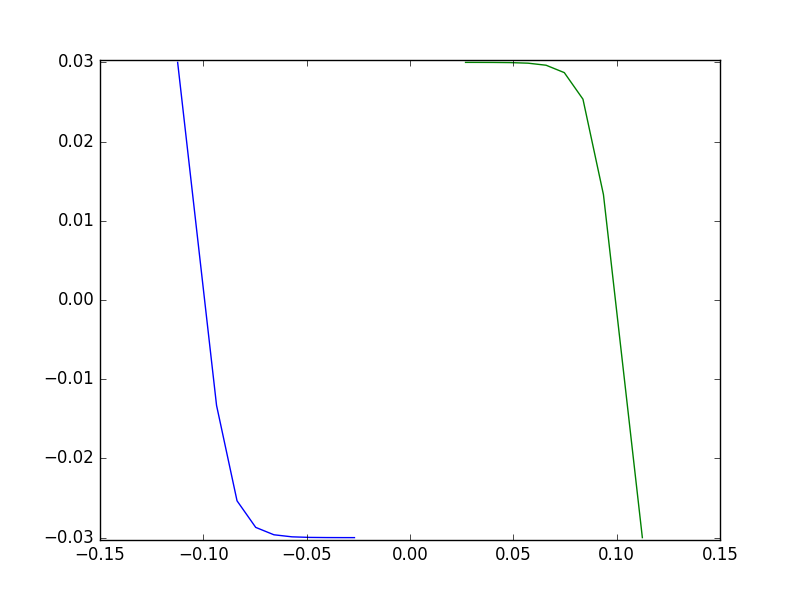
\includegraphics[width=0.8\linewidth]{impurity_levels.png}
    \end{minipage}
    \hfill
    \begin{minipage}[t]{0.45\linewidth}
        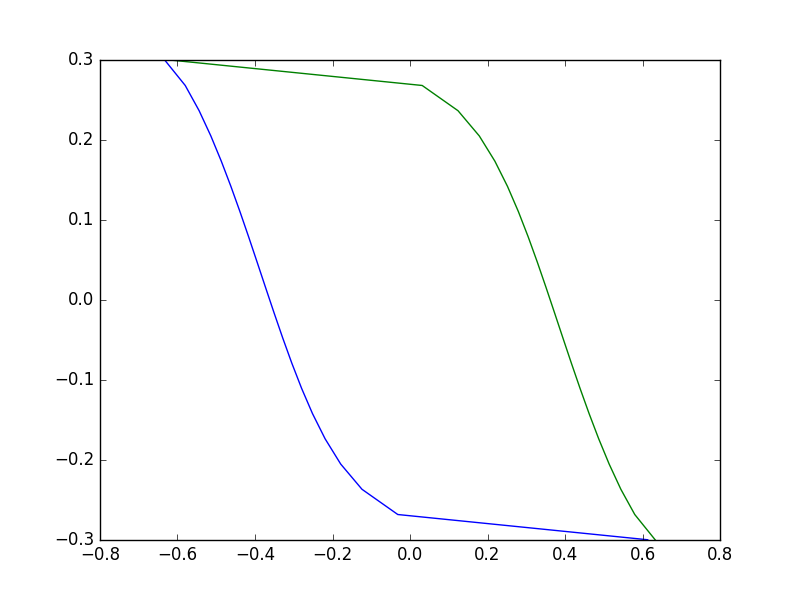
\includegraphics[width=0.8\linewidth]{gf_03-1-04.png}
    \end{minipage}
        \caption{
                На графиках показаны уровни энергии связанных состояний на точечной примеси
                для $m,t = 1,0.4$, $\xi = 0.03$ (слева), $\xi = 0.3$ (справа)
                По оси абсцисс отложена обратная глубина ямы, $\Delta E^{-1}$. Видно,
                что при бесконечной глубине ямы имеются два слабо связанных состояния.
                }
    \label{fig:impurity_numeric_levels}
\end{figure}

Заметим, что при определённых энергиях примеси связанные состояния лежат в середине 
зоны. Это значит, что они могут перекрываться с краевыми состояниями.
